\subsubsection{Photo-evaporation of a dense clump}
\label{sec.tests.raytracing}

\begin{figure}
  \centering
  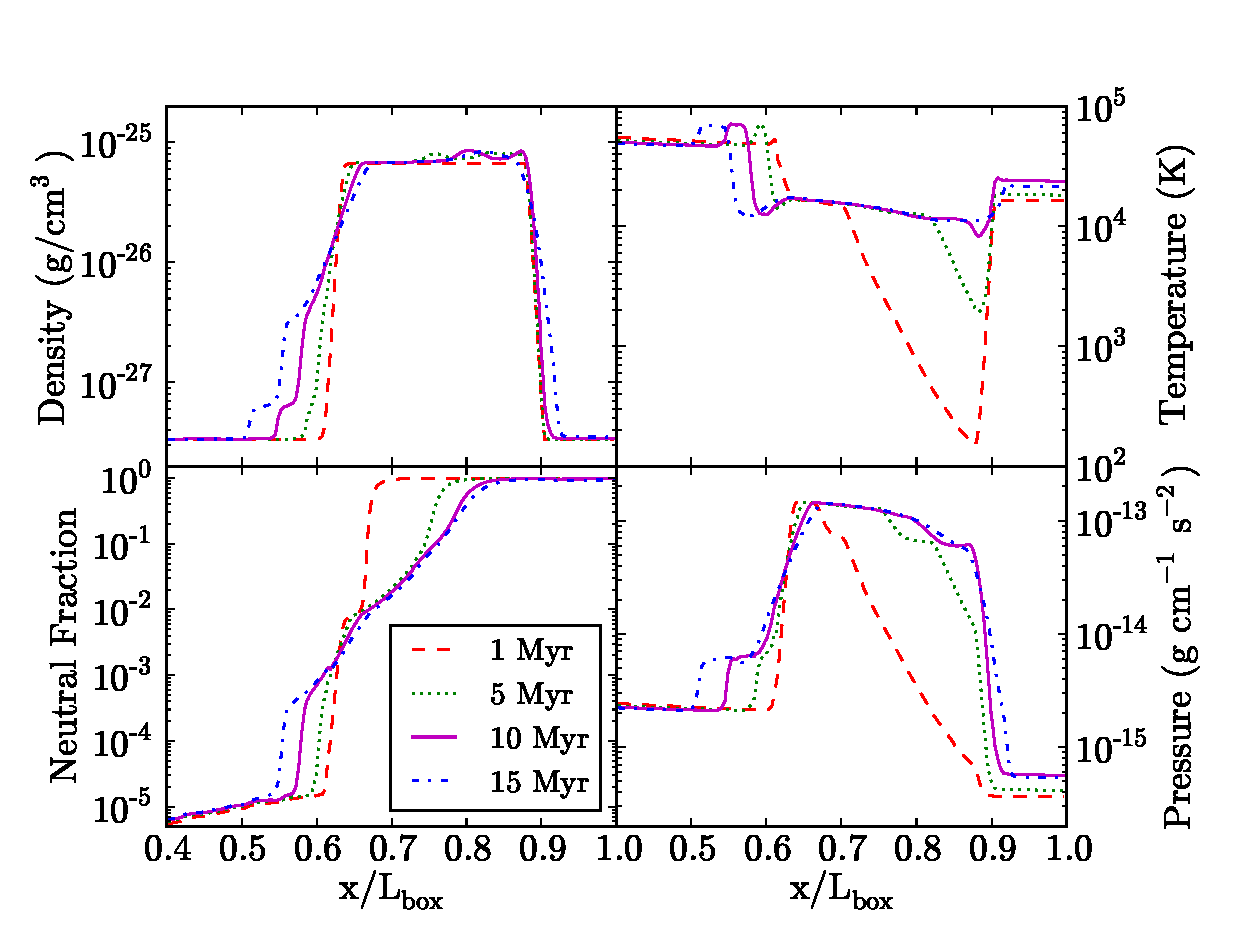
\includegraphics[width=0.48\textwidth]{figures/shadowing-rays.eps}
  \hfill
  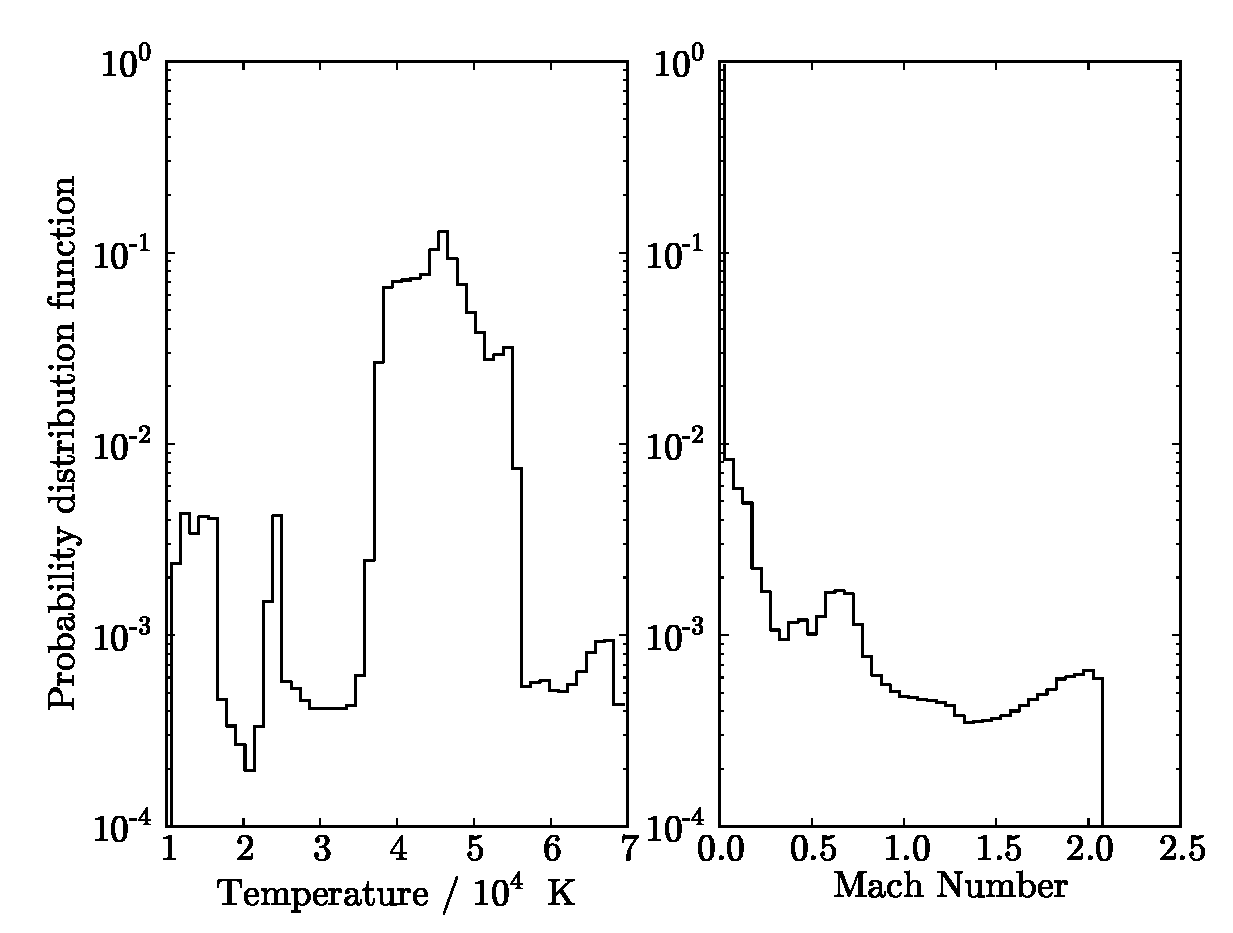
\includegraphics[width=0.48\textwidth]{figures/shadowing-pdf.eps}
  \caption{Photo-evaporation of a dense clump using the Moray
    ray-tracing module.  Left panel: Line cuts in the axis from the
    point source to the clump center at $t = 1, 5, 10, 15$~Myr
    (clockwise from the upper-left side) of the density, temperature,
    pressure, and neutral fraction.  Right panel: Volume-weighted
    probability distribution functions for the temperature (left-hand
    panel) and flow Mach number (right-hand panel) at $t = 10
    \unit{Myr}$.}
  \label{fig:shadowing1}
\end{figure}

\begin{figure}
  \centering
  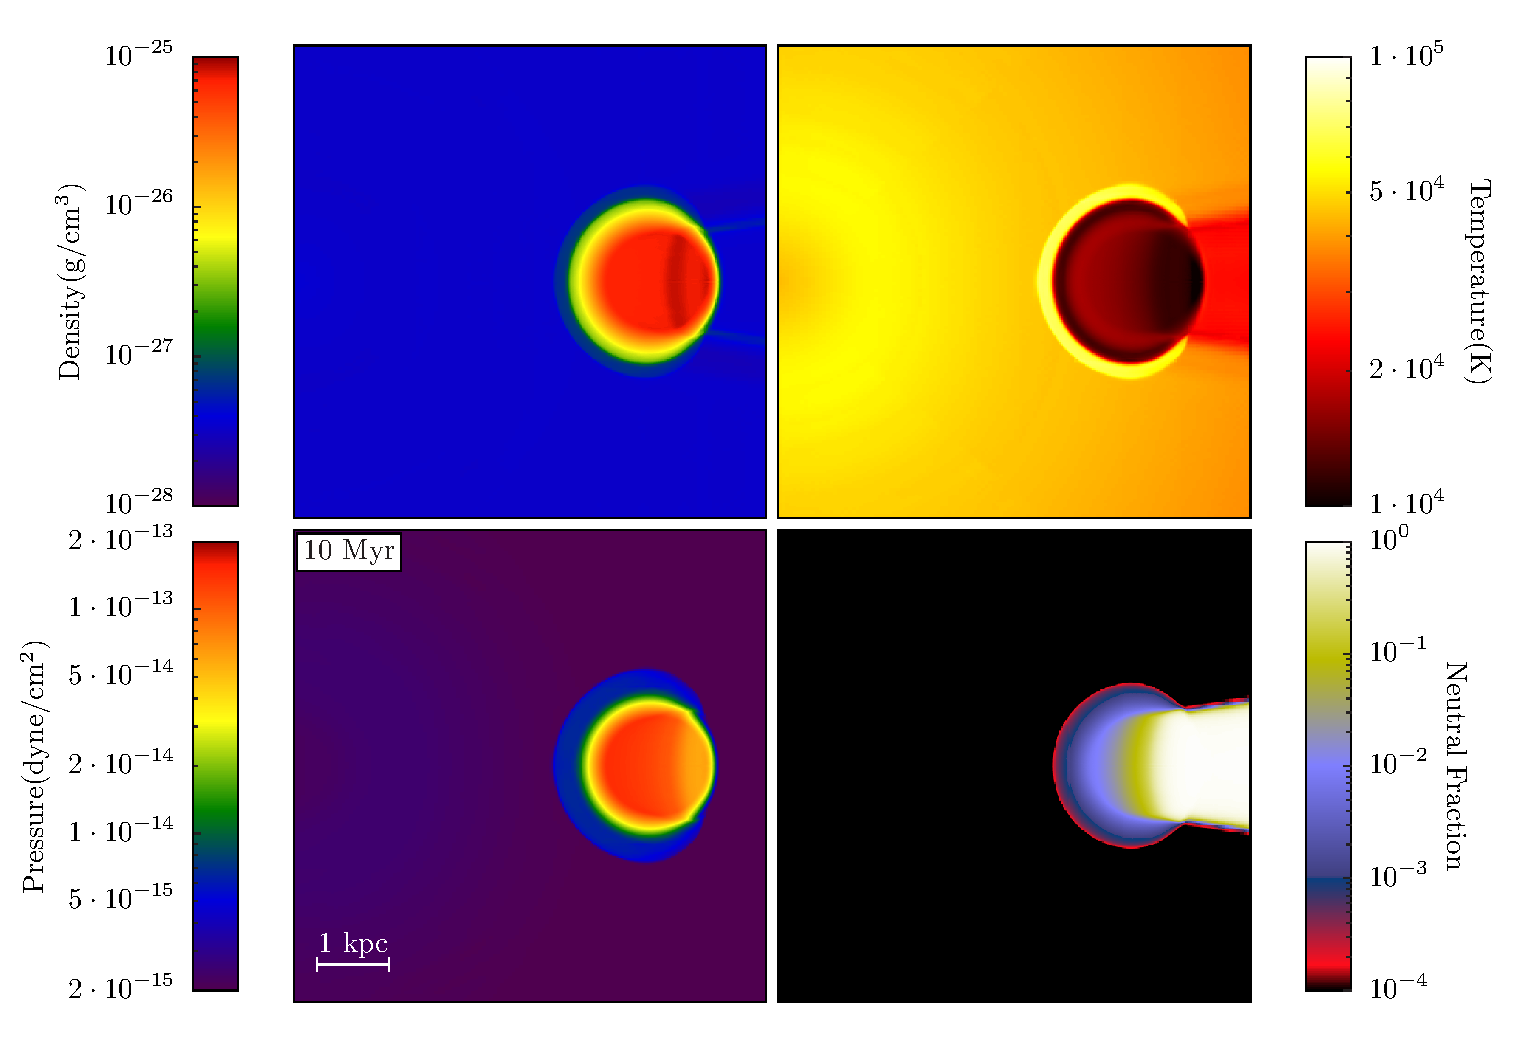
\includegraphics[width=1.0\textwidth]{figures/shadowing-slices.eps}
  \caption{Photo-evaporation of a dense clump using the Moray
ray-tracing module.  Clockwise from the upper left: slices
through the clump center of density, temperature, neutral hydrogen
fraction, and pressure at $t=10$~Myr after the initialization of the
simulation.  A point source of radiation is at the center of the -x
boundary and illuminates the clump with a constant luminosity, casting
a clear shadow behind the clump, as seen in the neutral hydrogen
fraction.}
  \label{fig:shadowing2}
\end{figure}

The photo-evaporation of dense clumps of gas is prevalent in radiation
hydrodynamics simulations, and this test problem examines the
ionization front propagation into a dense clump, shadowing effects
behind the clump, and the hydrodynamic response on the clump from
photo-heating, all using \enzo's Moray ray-tracing module.  The
problem setup is the same as Test 7 in the Cosmological Radiative
Transfer Comparison Project \citep{IlievEtAl2009} and
\citet{Wise11_Moray}.  The simulation domain is 6.6~kpc on a side with
an ambient medium of pure neutral hydrogen of density $n_{\rm H} = 2
\times 10^{-4}\; \cubecm$ and temperature $T = 8000 \unit{K}$.  We
place a spherical overdensity in hydrostatic equilibrium with the
ambient medium.  It has a radius $r = 0.8 \unit{kpc}$, hydrogen
density $n_{\rm H} = 0.04\ \cubecm$ (i.e., overdensity of 200), and
temperature $T = 40$ K, and is centered at $(x,y,z) = (5, 3.3, 3.3)
\unit{kpc}$.  In \citet{IlievEtAl2009} all of the codes used a fixed
$128^3$ grid to ease the comparison, but in this test to demonstrate a
higher resolution AMR solution, we employ a $128^3$ grid with two
additional levels of refinement by factors of 2 for cells with a
baryon mass greater than 1.5 (method 2 in
Section~\ref{sec:refinement_criteria}). This test is run for 15 Myr.

The cloud is subject to radiation from a point source at the center of
the $x=0$ boundary with an ionizing photon luminosity $\dot{N}_\gamma
= 3 \times 10^{51}$ photons s$^{-1}$, corresponding to a flux $F_0 =
10^6 \unit{photons s}^{-1} \unit{cm}^{-2}$ at the clump surface
closest to the radiation source.  The radiation source has a spectrum
of a $T = 10^5 \unit{K}$ blackbody, and we use four energy groups with
the following mean energies and relative luminosities: $E_i = (17.98,
31.15, 49.09, 76.98) \unit{eV}, L_i/L = (0.23, 0.36, 0.24, 0.06)$ that
are optimized to reduce errors in the solutions with a full spectrum
and energy discretization \citep{Mirocha12}.  (Note that this choice
of energy groups is different from those used in Wise \& Abel 2011.)
\nocite{Wise11_Moray} We use a minimum angular resolution of 10 rays
per cell and a constant radiative transfer timestep of 25 kyr.  

The left panel in Figure \ref{fig:shadowing1} shows cuts of the
density, temperature, neutral fraction, and pressure in a line
connecting the source and the clump center at $t = 1, 5, 10, 15$~Myr.
At 1~Myr, the ionization front has propagated through the leftmost
500~pc of the clump.  This heated gas is now overpressurized, as seen
in the pressure plot of Figure \ref{fig:shadowing1} that expands into
the ambient medium.  This photo-evaporative flow becomes apparent at
5~Myr with the increased density and pressure on the left side of the
clump.  The right panel in Figure \ref{fig:shadowing1} shows the
volume-weighted distributions of the temperature and flow Mach number
in the entire domain at $t = 10 \unit{Myr}$.  Overall, our results
agree well with the codes presented in \citet{IlievEtAl2009} and the
uniform grid test of \moray~\citep{Wise11_Moray}.

However, there are some small differences in the line cuts and
distributions that arise from our choice of energy discretization that
better samples the high-energy tail of a $T = 10^5 \unit{K}$ blackbody
spectrum and does not signify possible shortcomings of \moray.  First,
in the temperature cut at $t = 10 \unit{Myr}$, the high-energy
radiation photo-heat the gas to $T = 10^4 \unit{K}$, but it remains
primarily neutral.  The temperature dip at $x \simeq 0.88$ is the gas
has not come into thermal equilibrium with the incident radiation.  A
stronger temperature dip exists in the \citeauthor{IlievEtAl2009}
results and varies from 1000 to 8000~K between codes.  Another minor
difference is the larger breadth in the temperature distribution
feature centered at $T = 4.5 \times 10^4 \unit{K}$ that corresponds to
the ambient medium.  This difference also originates from the
different sampling in the spectral energy distribution of the source.
Figure \ref{fig:shadowing2} depicts the same quantities in a
two-dimensional slice through the clump center at $t = 10$ Myr.  At
this time, it is apparent that the outer layers are expanding after
being photo-heated.  These slices also show the sharp shadowing
effects of the dense clump in the neutral fraction plot that is
representative of ray tracing techniques.
